\usetikzlibrary{calc}
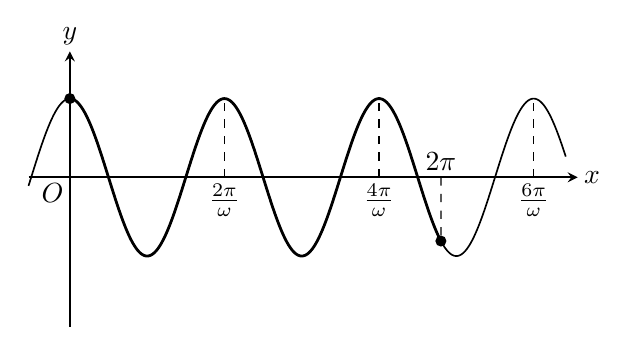
\begin{tikzpicture}[x=0.75cm,y=1.0cm,line width=.6pt,>=stealth,font=\normalsize]
% representative omega0=2.5 in [2,3); tick abscissae keep exact ratios:
% 2pi/w=2.6179938780, 4pi/w=5.2359877560, 2pi=6.2832, 6pi/w=7.8539816340
\draw[->,black] (-0.7,0)--(8.6,0) node[right,inner sep=0pt,xshift=2pt] {$x$};
\draw[->,black] (0,-1.9)--(0,1.6) node[above,inner sep=0pt,yshift=2pt] {$y$};
% full cosine y=cos(2.5x)
\draw[black,domain=-0.7:8.4,samples=300] plot (\x,{cos(deg(2.4*\x))});
% highlight interval [0,2pi] with thicker stroke (grayscale emphasis)
\draw[black,line width=1.0pt,domain=0:6.2831853072,samples=220] plot (\x,{cos(deg(2.4*\x))});
% dashed peak guides
\draw[black,dashed,line width=.45pt] (2.6179938780,0)--(2.6179938780,1);
\draw[black,dashed,line width=.45pt] (5.2359877560,0)--(5.2359877560,1);
\draw[black,dashed,line width=.45pt] (7.8539816340,0)--(7.8539816340,1);
\draw[black,dashed,line width=.45pt] (6.2832,0)--(6.2831853072,-0.8090169944);
% endpoint dots
\fill[black] (0,1) circle (2pt);
\fill[black] (6.2831853072,-0.8090169944) circle (2pt);
% ticks
\node[anchor=north east,inner sep=0pt,xshift=-2pt,yshift=-2pt] at (0,0) {$O$};
\node[anchor=north,inner sep=0pt,yshift=-2pt] at (2.6179938780,0) {$\frac{2\pi}{\omega}$};
\node[anchor=north,inner sep=0pt,yshift=-2pt] at (5.2359877560,0) {$\frac{4\pi}{\omega}$};
\node[anchor=south,inner sep=0pt,yshift=2pt] at (6.2832,0) {$2\pi$};
\node[anchor=north,inner sep=0pt,yshift=-2pt] at (7.8539816340,0) {$\frac{6\pi}{\omega}$};
\end{tikzpicture}
